\chapter{FOPT 3}

\section{Einführung in UML}

\textbf{UML} (\textit{Unified Modeling Languag}) ist eine grafische Notation zur Modellierung von Software\footnote{
die Spezifikationen sind zu finden unter \url{https://www.omg.org/spec/UML/} - abgerufen 28.01.2024
}.\\

\noindent
UML erlaubt die Modellierung unterschiedlicher Sichten auf ein Software-System, z.B

\begin{itemize}
    \item die \textbf{funktionalen Anforderungen} durch \textbf{Use Cases})
    \item die \textbf{statische Struktur}, {bspw.} strukturierende Einheiten wie Klassen und Packages und deren Beziehungen zueinander über Klassen- und Komponentendiagramme
    \item das dynamische VErhalten eines Systems, also zur Laufzeit, {bspw.} durch \textbf{Sequenzdiagramme}, \textbf{Aktivitätsdiagramme} und Diagramme für \textbf{endliche Automaten}
\end{itemize}
\noindent

\subsection{Klassendiagramme}

\textbf{Klassendiagramme} beschreiben die statische Struktur eines Programms und spiegeln in abstrakter Form den Quellcode des Programms wider.\\

\noindent
Wesentliche Einheiten: Klassen, Schnitstellen und deren Beziehungen zueinander.\\

\noindent
Symbole für Sichtbarkeiten in einem Klassendiagramm:

\begin{itemize}
    \item \code{public}: \code{+}
    \item \code{private}: \code{-}
    \item \code{protected}: \code{#}
\end{itemize}\\

\noindent
Ein Klassendiagramm besteht aus 3 vertikal angeordneten Blöcken:\\

\begin{enumerate}
    \item Klassenname / Schnittstellenname
        \begin{itemize}
            \item abstrakte Klassen werden kursiv geschrieben
            \item wenn es sich um ein Interface handelt, kann zur Kenntlichmachung ein \code{<<interface>>} über den Klassennamen gesetzt werden
        \end{itemize}
    \item Attribute
        \begin{itemize}
            \item[] \code{[Sichtbarkeit] [Name]:[Typ]}
        \end{itemize}
    \item Methoden
    \begin{itemize}
        \item[] \code{[Sichtbarkeit] [Name]([Parameterliste]):[Rückgabetyp]}
        \item[] \code{Parameterliste}: \code{[Name]:Typ}, kommasepariert
    \end{itemize}
\end{enumerate}\\

\noindent
\underline{Statische Attribute und Methoden werden unterstrichen.}\\

\noindent
Klassen und Schnittstellen, die zu einem \textbf{Package} gehören, können in einem Rechteck zusammengefasst werden, das mit dem Package-Namen beschriftet ist\footnote{
Das Skript FOPT3 weist auf Seite 3 darauf hin, das in dem Kurs i.d.R. Klassendiagramme ohne Attribute und Methoden dargestellt werden. Das Rechteck beinhaltet dann nur den Klassennamen.
}.

\begin{figure}
    \centering
    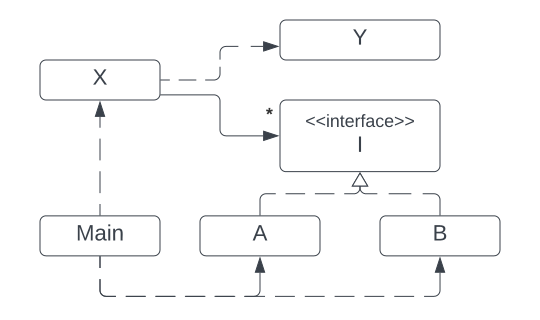
\includegraphics[scale=0.5]{chapters/fopt3/img/classdiagram}
    \caption{Ein Beispiel für ein UML-Klassendiagramm. (Quelle: eigene)}
    \label{fig:classdiagram}
\end{figure}

\subsection{Assoziationen}

Ein Attribut, das vom Typ einer Schnittstelle oder einer Klasse ist, kann durch eine \textbf{Assoziation} dargestellt werden.\\

\noindent
Assoziationen sind einfache Pfeile, die in Richtung der verwendeten Klasse/ Schnittstelle zeigen, die das Attribut darstellt.\\

\noindent
Klassendiagramme sind statisch; eine mögliche Dynamik kann über \textbf{Kardinalitäten} dargestellt werden.\\
In der folgenden Abbildung~\ref{fig:association} referenziert im Beispiel b) ein \code{Company}-Objekt genau ein oder kein \code{Employee}-Objekt.\\
Im Beispiel c) referenziert ein \code{Company}-Objekt genau ein \code{Employee}-Objekt.\\

\noindent
Werden mehrere \code{Employee}-Objekte zur Laufzeit erzeugt, kann man die deren Beziehungen zu den \code{Company}-Objekten ebenfalls durch Kardinalitäten ausdrücken:\\
\noindent
Im Beispiel d) wird ein \code{Employee}-Objekt von mehreren \code{Company}-Objekten referenziert.\\
\noindent
Im Beispiel e) wird ein \code{Employee}-Objekt immer von genau einem \code{Company}-Objekt referenziert.

\begin{figure}
    \centering
    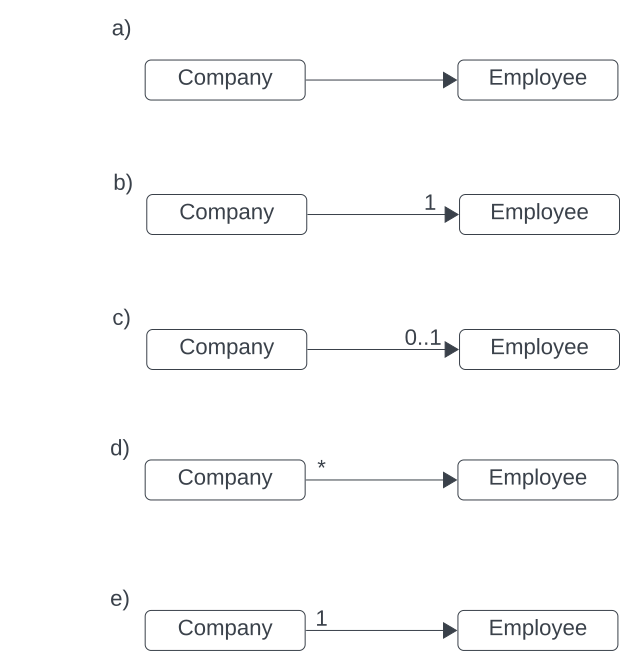
\includegraphics[scale=0.5]{chapters/fopt3/img/association}
    \caption{Beispiele für Assoziation mit Kardinalitäten. (Quelle: eigene)}
    \label{fig:association}
\end{figure}

\noindent
In dem folgenden Beispiel kann ein \code{Company}-Objekt mehrere \code{Employee}-Objekte referenzieren:

\begin{figure}
    \centering
    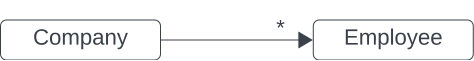
\includegraphics[scale=0.5]{chapters/fopt3/img/multipleemployees}
    \caption{Ein Company-Objekt referenziert mehrere Employee-Objekte. (Quelle: eigene)}
    \label{fig:multipleemployees}
\end{figure}

Im Code lässt sich das bspw. folgendermaßen umsetzen:
\newpage

\begin{minted}[mathescape,
    linenos,
    numbersep=5pt,
    gobble=2,
    frame=lines,
    framesep=2mm]{java}
    public class Company {

        private List<Employee> employees;

        public Company() {
            employees = new ArrayList<Employee>();
        }

    }
\end{minted}\\

\subsection{Objektdiagramme}

\textbf{Objektdiagramme} beschreiben eine Situation zu einem bestimmten Zeitpunkt.\\

\noindent
Objekte werden durch ein Rechteck dargestellt, in der ein \underline{unterstrichenes} \code{:[Klassenname]} die Instanz repräsentiert. \\
In dieser Schreibweise wird eine anonyme Instanz repräsentiert.
Wird hingegen ein Bezeichner vor den Doppelpunkt gestellt, wird auf ein konkretes Objekt verwiesen.\\

\begin{figure}
    \centering
    
\includegraphics[scale=0.5]{chapters/fopt3/img/objectdiagram}
    \caption{Beispiel für ein Objektdiagram (ohne Attribute und Methoden). (Quelle: eigene)}
    \label{fig:objectdiagram}
\end{figure}

\noindent
Verschiedene Assoziationen von Objekten sind in Abbildung~\ref{fig:objectassociations} dargestellt.\\
In dem Beispiel b) referenziert eine \code{Company} mehrere \code{Employee}s.\\
Im Beispiel c) wird ein \code{Employee} von mehreren \code{Company}s referenziert.\\

\begin{figure}
    \centering
    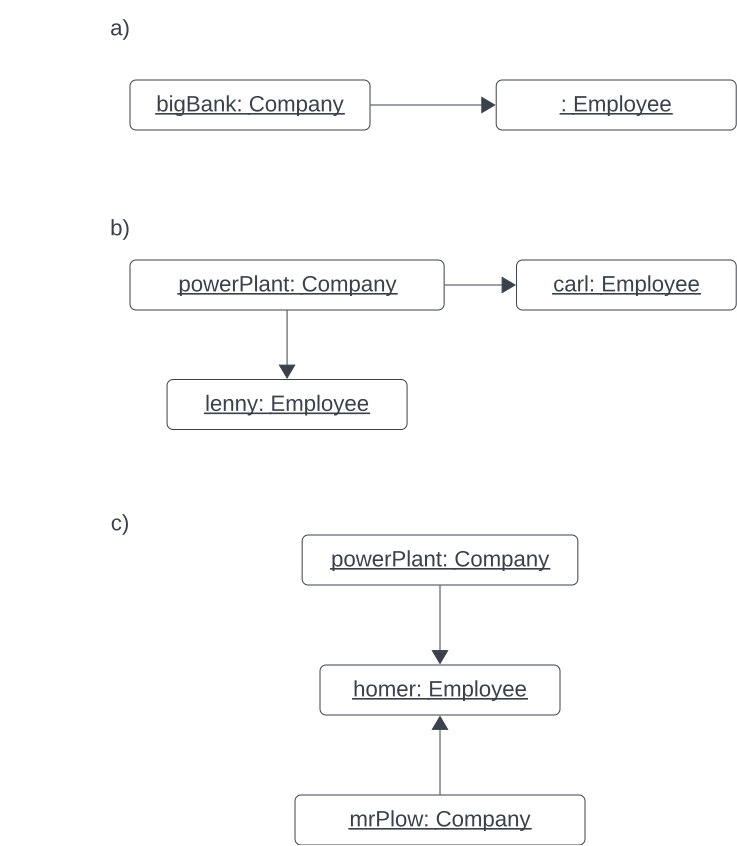
\includegraphics[scale=0.5]{chapters/fopt3/img/objectassociations}
    \caption{Beispiele für Assoziationen bei Objektdiagrammen. (Quelle: eigene)}
    \label{fig:objectassociations}
\end{figure}

\noindent
$\rightarrow$ Objektdiagramme sind nur zu einem bestimmten Zeitpunkt während des Ablaufs eines Programms gültig.\\

\noindent
$\rightarrow$ In einem Klassendiagramm modelliert man die Aspekte, die bei einer bestimmten Betrachtung betont werdne sollen.\\

\noindent
Es ist auch möglich, Assoziationen in beide Richtungen zu modellieren:

\begin{figure}
    \centering
    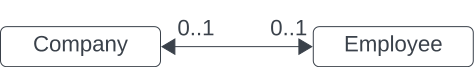
\includegraphics[scale=0.5]{chapters/fopt3/img/bidirectionalassociation}
    \caption{Beispiel für eine bidirektionale Assoziation. (Quelle: eigene)}
    \label{fig:bidirectionalassociation}
\end{figure}

Im Code lässt sich das bspw. folgendermaßen umsetzen:
\newpage

\begin{minted}[mathescape,
    linenos,
    numbersep=5pt,
    gobble=2,
    fontsize=\small,
    frame=lines,
    framesep=2mm]{java}
    public class Company {
        private Employee emp;
    }
    public class Employee {
        private Company comp;
    }
\end{minted}\\

\noindent
    Bei einer bidirektionalen Assoziation, die über ein Klassendiagramm modelliert ist, muss nicht unbedingt die Instanz auf die referenzierende Instanz zurückverweisen - hierbei kann es sich auch um ein unterschiedliches Objekt handeln.\\

\begin{figure}
    \centering
    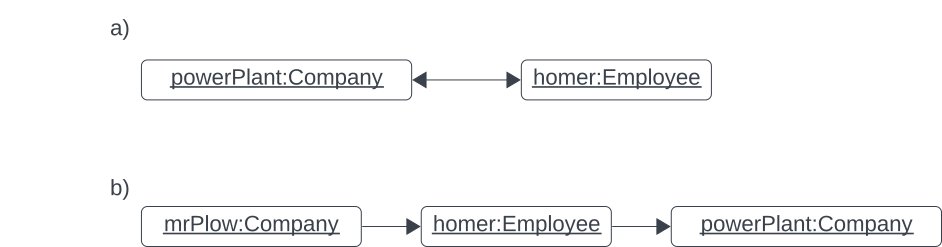
\includegraphics[scale=0.5]{chapters/fopt3/img/bidirectionalassocexample}
    \caption{Beispiele für bidirektionale Assoziation. In b) ist die Situation dargestellt, bei denen auf die referenzierende Klasse nicht unbedingt von der referenzierten Klasse zurückverwiesen werden muss. (Quelle: eigene)}
    \label{fig:bidirectionalassocexample}
\end{figure}

Die Situation aus Abbildung~\ref{fig:bidirectionalassocexample} b) kann wie folgt im Code implementiert werden.

\begin{minted}[mathescape,
    linenos,
    numbersep=5pt,
    gobble=2,
    frame=lines,
    framesep=2mm]{java}
    Company powerPlant = new Company();
    Company mrPlow = new Company();
    Employee homer = new Employee();

    powerPlant.setEmployee(homer);
    homer.setCompany(mrPlow);
\end{minted}\\

\noindent
Assoziationen können auch \textbf{reflexiv} sein;


\begin{figure}
    \centering
    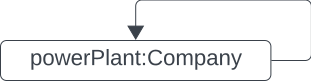
\includegraphics[scale=0.5]{chapters/fopt3/img/reflexive}
    \caption{Beispiel für eine Klasse, die sich selbst referenziert. Die Refenz muss nicht unbedingt auf dieselbe Instanz verweisen, aber zumindest auf denselben Typen. (Quelle: eigene)}
    \label{fig:reflexive}
\end{figure}


\subsection{Benutzt-Beziehungen}

\begin{tcolorbox}
    Referenzen, die einen Methodenaufruf nicht überdauern (Parameter, Rückgabe, lokale Variable), werden durch \textbf{Benutzt-Beziehungen} ausgedrückt.\\

    \noindent
    Eine \textbf{Assoziation} schließt eine \textbf{Benutzt-Beziehung} imemr mit ein.
\end{tcolorbox}\\

\noindent
Wenn eine Klasse \code{X} kein Attribut vom Typ \code{Y} benutzt, kann die Klasse \code{Y} dennoch von \code{X} verwendet werden, bspw. bei Methoden als Übergabeparameter, als Rückgabetyp oder als lokale Variable.\\

\noindent
Eine \textbf{Benutzt-Beziehung} wird durch eine gestrichelte Linie dargestellt.\footnote{
Das Skript zu FOPT 3 geht bei der Benutzt-Beziehung nicht sehr in die Tiefe, auch wird i.d.R. eine gestrichelte Pfeilspitze anstatt einer geschlossenen für die Benutzt-Beziehungen verwendet. Siehe hierzu auch die UML-Spezifikation unter \url{https://www.omg.org/spec/UML/2.5.1/PDF} - abgerufen 28.01.2024
}
In Abbildung

\begin{figure}
    \centering
    
\includegraphics[scale=0.5]{chapters/fopt3/img/uses}
    \caption{Beispiel für eine Benutzt-Beziehung unter Verwendung der Notation aus dem FOPT 3 Skript. (Quelle: eigene)}
    \label{fig:uses}
\end{figure}

\subsection{Vererbungs- und Implementierungsbeziehungen}

\textbf{Vererbungsbeziehungen} werden durch einen offenen Pfeil und eine durchgezogene Linie Richtung der Elternklasse dargestellt (s. Abbildung~\ref{fig:inheritance} a).\\

\textbf{Implementierungsbeziehungen} werden durch einen offenen Pfeil und eine gestrichelte Linie Richtung der implementierten Schnittstelle dargestellt (s. Abbildung~\ref{fig:inheritance} b).\\

In Java können Schnittstellen gleichzeitig von mehreren Schnittstellen erben, was in (s. Abbildung~\ref{fig:inheritance} b) dargestellt ist.\\

\begin{minted}[mathescape,
    linenos,
    numbersep=5pt,
    gobble=2,
    frame=lines,
    framesep=2mm]{java}
    public Interface A extends B, C {
        ...
    }
\end{minted}\\

\begin{figure}
    \centering
    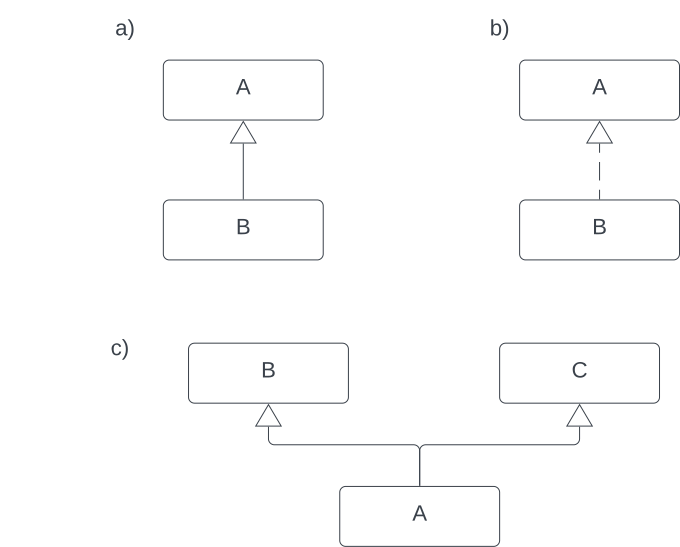
\includegraphics[scale=0.5]{chapters/fopt3/img/inheritance}
    \caption{Beispiele für Vererbungs- und Implementierungsbeziehungen. (Quelle: eigene)}
    \label{fig:inheritance}
\end{figure}


\subsection{Sequenzdiagramme}

\textbf{Sequenzdiagramme} dienen zur grafischen Beschreibung des dynamischen Verhaltens eines Programmes.\\

\begin{tcolorbox}
\blockquote[{\cite[333]{Oes05}}]{
Der Zweck von Sequenzdiagrammen ist es, genau ein Szenario darzustellen und nicht eine Menge von verschiedenen Abläufen.
}
\end{tcolorbox}

\noindent
Sequenzdiagramme werden auch \textbf{Raum-Zeit-Diagramme} genannt, weil auf der $x$-Achse der Raum der involvierten
Objekte dargestellt wird, während die $y$-Achse nach unten die Zeit symbolisiert.\\

\noindent
Als Beispiel sei folgender Code gegeben, der in dem Sequenzdiagramm in Abbildung~\ref{fig:sequence} dargestellt ist.

\begin{minted}[mathescape,
    linenos,
    numbersep=5pt,
    gobble=2,
    frame=lines,
    framesep=2mm]{java}
    class X {
        public void foo(Y y) {
            y.bar();
        }
    }
    public class SequenceDemo {
        X x;
        Y y;
        public static void main(String[] args) {
            x = new X();
            y = new Y();
            x.foo(y);
        }
    }
\end{minted}\\


\begin{figure}
    \centering
    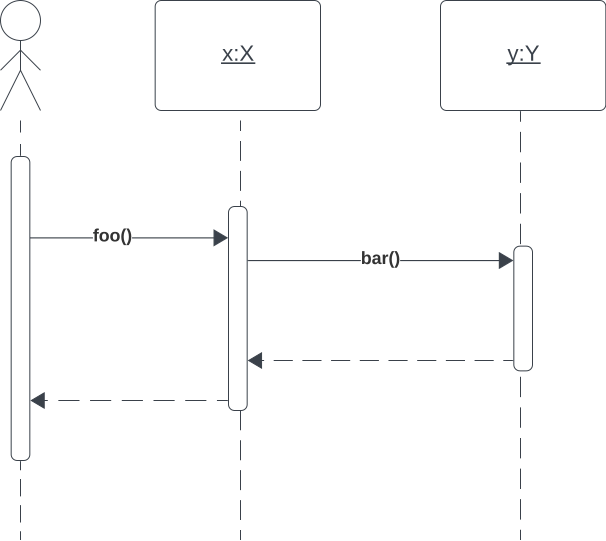
\includegraphics[scale=0.5]{chapters/fopt3/img/sequence}
    \caption{Beispiel für ein Sequenzdiagramm. (Quelle: eigene)}
    \label{fig:sequence}
\end{figure}

\noindent
Die Kästchen auf der $x$-Achse symbolisieren \textbf{Objekte}, \underline{nicht} Klassen.\\

\noindent
Gestrichelte Linien stellen die Lebenszeit der involvierten Objekte dar.\\

\noindent
Aufruf einer Methode wird durch eine durchgezogene Linie gekennzeichnet, die Rückkehr aus der Methode durch eine
gestrichelte Linie.\\

\noindent
Ein Sequenzdiagramm gibt immer einen von mehreren möglichen Abläufen an.\\

\noindent
Findet ein Methodenaufruf bei einem Objekt statt, auf dem bereits ein Methodenaufruf stattfindet, wird das Kästchen für den Methodenaufruf leicht versetzt dargestellt, wie im folgenden Beispiel zu sehen ist (s. Abbildung~\ref{fig:callback}).

\begin{minted}[mathescape,
    linenos,
    numbersep=5pt,
    gobble=2,
    frame=lines,
    framesep=2mm]{java}

    class Y {
        public void bar(X x) {
            x.callback();
        }
    }

    class X {
        public void foo(Y y) {
            y.bar(this);
        }

        public void callback() {
            ...
        }
    }
    public class SequenceDemo {
        X x;
        Y y;
        public static void main(String[] args) {
            x = new X();
            y = new Y();
            x.foo(y);
        }
    }
\end{minted}\\

\begin{figure}
    \centering
    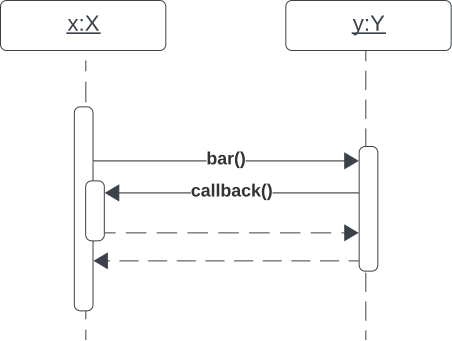
\includegraphics[scale=0.5]{chapters/fopt3/img/callback}
    \caption{Beispiel für ein Sequenzdiagramm, bei dem eine Methode des aufrufenden Objektes aufgerufen wird. (Quelle: eigene)}
    \label{fig:callback}
\end{figure}

\noindent
Die Darstellung \textbf{rekursiver Aufrufe} ist ebenfalls möglich, wie Abbildung~\ref{fig:recursion} zeigt:

\begin{figure}
    \centering
    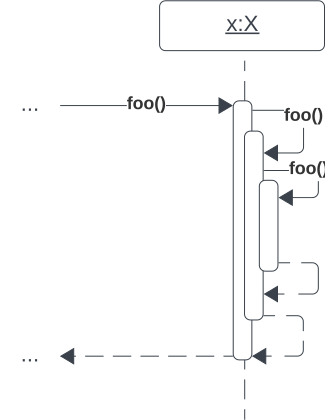
\includegraphics[scale=0.5]{chapters/fopt3/img/recursion}
    \caption{Beispiel für ein Sequenzdiagramm für rekursive Aufrufe der Methode foo(). (Quelle: eigene)}
    \label{fig:recursion}
\end{figure}


\noindent
Werden erst während der Abfolge eines Sequenzdiagramms neue Objekte erzeugt, werden diese Objekte in dem Sequenzdiagramm versetzt dargestellt, wie Abbildung~\ref{fig:create} illustriert:

\begin{figure}
    \centering
    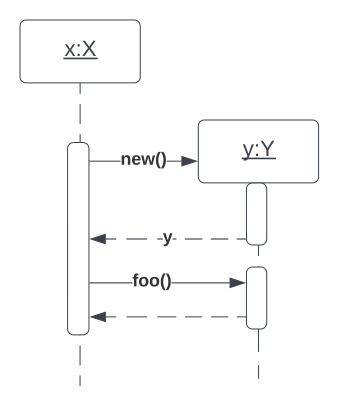
\includegraphics[scale=0.5]{chapters/fopt3/img/create}
    \caption{Beispiel für die Darstellung der Erzeugung eines neuen Objektes in einem Sequenzdiagramm. (Quelle: eigene)}
    \label{fig:create}
\end{figure}
